\documentclass{book}
\title{A Computational Tour of Number Theory}
\author{William Stein \and Andrew Ohana \and Simon Spicer \and Hao Chen
\and Yannick Van Huele \and Bharath \and Travis Scholl \and ADD/FIX YOUR NAME! }

\usepackage{macros}

\begin{document}
\maketitle
\tableofcontents

\chapter{Introduction: tour of the main questions}
In this book, we will explore several important central problems and
objects of number theory, and for each to explain how---in practice
(not just theory)---to {\em compute} with them.    Books,
papers, and web sites such as Wikipedia and Mathoverflow often
give excellent descriptions
of mathematical objects, algorithms, data, conjectures, and theorems.
However, they rarely give concrete instructions
so that you can manipulate them on a computer, with enough theoretical
discussion so that you understand the limitations and capabilities of
your tools.  That is the mission of the book you are looking at.


\section{Prime Numbers}
The prime numbers $2,3,5,7,11,\ldots, $ have fascinated
mathematicians for thousands of years.  Euclid proved there
are infinitely many: if $p_1,\ldots, p_n$ are primes,
then $p_1\cdots p_n + 1$ is an integer divisible by some
prime $p$ that isn't equal to any $p_i$.

Let's compute the primes up to 100:
\begin{lstlisting}
sage: prime_range(100)
[2, 3, 5, 7, 11, 13, 17, 19, 23, 29, 31, 37, 41, 43, 47, 53, 59, 61, 67, 71,
 73, 79, 83, 89, 97]
\end{lstlisting}
And draw a plot of the function $\pi(x)$ that counts the number of primes
up to $x$ for $x<100$.
\begin{center}
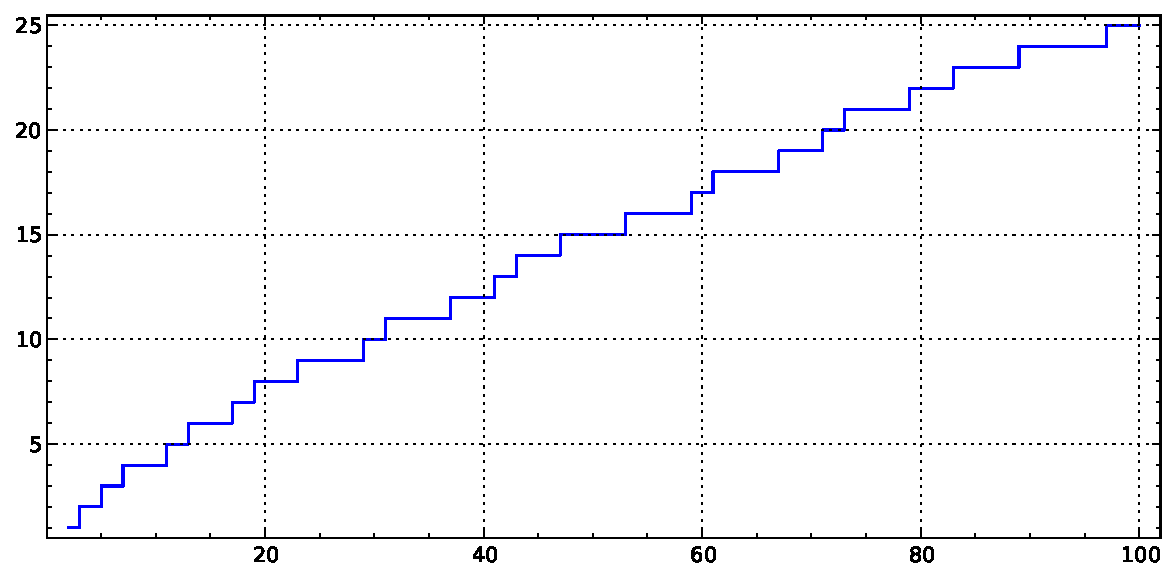
\includegraphics[width=.7\textwidth]{pics/prime_pi-2-100.pdf}
\end{center}

The {\em Prime Number Theorem}, which was proved over a century ago, asserts
that $\pi(x) \sim x/\log(x)$:

\begin{lstlisting}
@interact
def f(B=[10^n for n in [2..9]]):
    show(plot(lambda x: prime_pi(x)/(x/log(x)), (x,2,B))
       + line([(0,1),(B,1)],color='red'))
\end{lstlisting}

\begin{center}
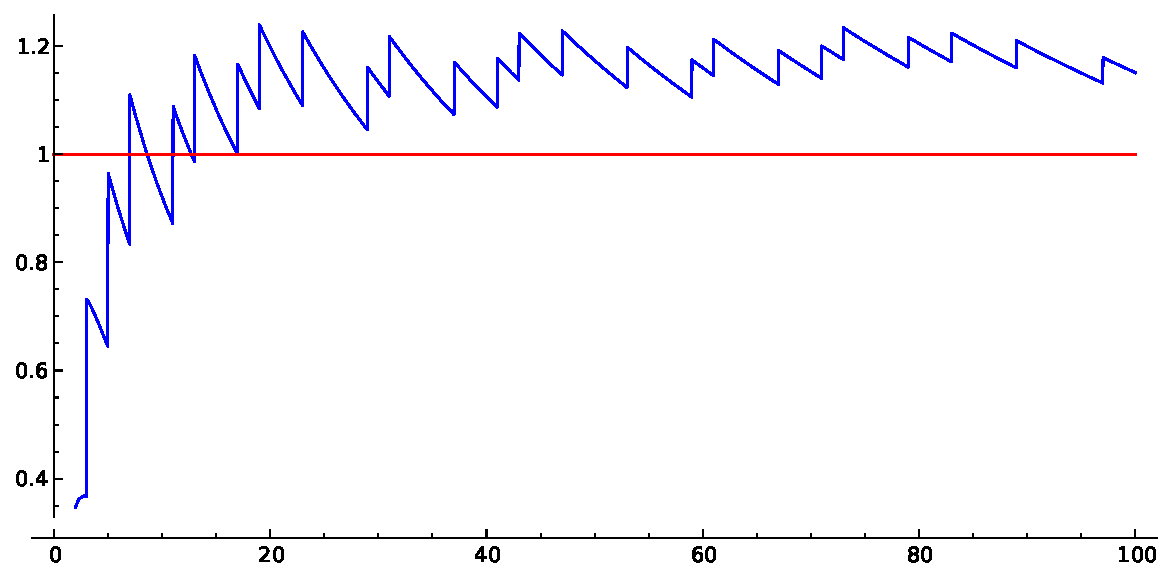
\includegraphics[width=.3\textwidth]{pics/pnt100.pdf}
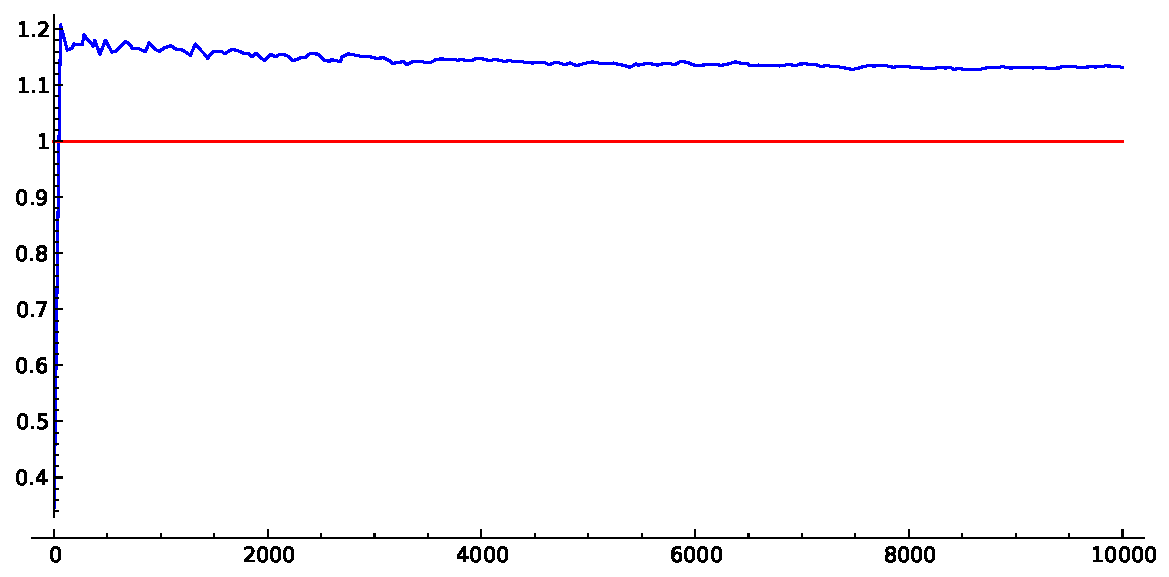
\includegraphics[width=.3\textwidth]{pics/pnt10000.pdf}
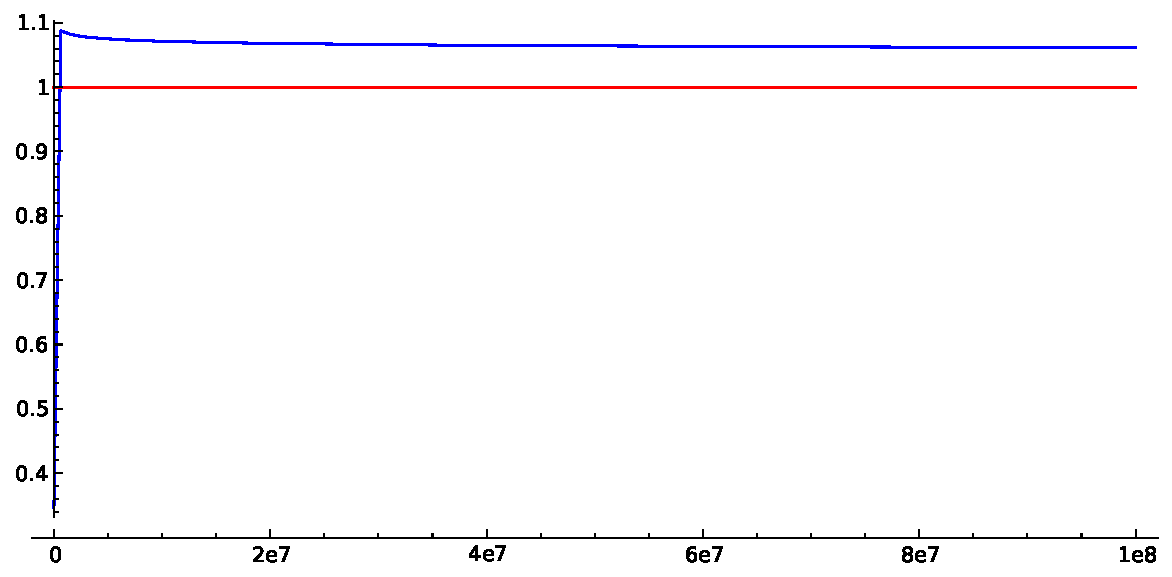
\includegraphics[width=.3\textwidth]{pics/pnt100000000.pdf}
\end{center}

The {\em Riemann Hypothesis}, which remains completely unsolved today,
asserts that for all $x\geq 2.01$,
$$
 |\pi(x) - \Li(x)| \leq \sqrt{x}\cdot \log(x),
$$
where
$$
 \Li(x) = \int_{2}^x \frac{dt}{\log(t)}
$$

In the range of the following plots, $\pi(x) - \Li(x)$ is
much smaller than $\sqrt{x}\log(x)$.
\begin{lstlisting}
@interact
def f(B=[10^n for n in [2..9]]):
    print "sqrt(B)*log(B) = ", round(sqrt(B)*log(B))
    show(plot(lambda x: prime_pi(x) - Li(x), (x,2,B)))
\end{lstlisting}
\begin{center}
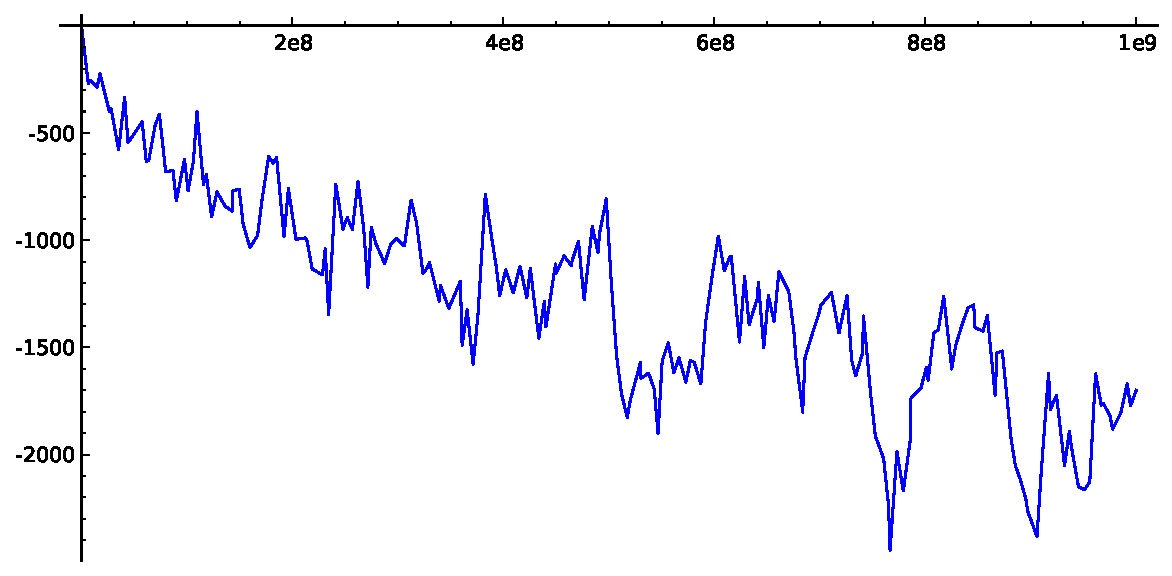
\includegraphics[width=.7\textwidth]{pics/pi_minus_li-1e9.pdf}
\end{center}
Up to $10^9$ we have $|\pi(x)-\Li(x)|$ is much
smaller than $\sqrt{10^9}\cdot \log(10^9) \sim  \num{655327}$.

\hw{Andrew and Bharath}{Can we prove anything toward $\sqrt{x}\cdot \log(x)$?}

% Basic calculus bound by Bharath
One can follow a naive approach and use basic calculus.
One sees easily that $\pi(x) \leq x$. Similarly, If $x \geq 2$, then $\log(x) \geq \log(2)$. So, we have that $\Li(x) \leq \frac{x}{log(2)} $.
Using triangular inequality, one can deduce that $|\pi(x)-\Li(x)| \leq x \cdot (1 + \frac{1}{\log(2)}) \leq 3x$.


\section{Class Numbers}
Number fields are a natural generalization of the rational numbers $\Q$,
to which ideas such as primes, and conjectures such as
the Riemann Hypothesis, etc., all generalize.  They have
been intensely studied, initially motivated by
work to prove Fermat's Last Theorem.

In this book we will assume you know abstract algebra; however,
as a quick reminder, an {\em ideal} $I$ in a commutative ring $R$ is an
additive subgroup of $R$ such that for all $x\in R$ we have $xI \subset I$.
A {\em number field} $K$ is a finite algebraic extension of
the rational numbers $\Q$; equivalently, it is a field obtained
by adjoining a root $\alpha$ of some polynomial $f(x) \in \Q[x]$.
The {\em ring of integers} $R=\O_K$ of a number field $K$ is the
set of all $\alpha\in K$ such that $\alpha$ is a root of some
monic polynomial $f(x)\in\Z[x]$.  It is interesting to prove
that $R$ (as defined) is closed under addition and multiplication
(it is a ring).
In the special case when $K=\Q$, we have $R=\Z$.

\subsection{Proof that the ring of integers is a ring}
%\hw{Volunteer!}{Put a proof or good ref to proof in as a footnote.}
%Yannick: Added a sketch of proof.  Still need to include the reference and
%merge with the preceding paragraph.  It may also be worth discussing
%$\bar{\Q}$ in a little more detail.
As the name suggests, the ring of integers of a number field is in fact a ring.
(Note, for example, that when $K = \Q$, the ring of integers is simply
$\O_K = \Z$.)
A sketch of the proof is given below.
A more detailed
exposition can be found in sections 2.2 and 2.3 of \cite{stein:ant}.

To prove that $\O_K$ is a ring, let us first define a related object:  Fix
an algebraic closure $\bar{\Q}$ of the rational numbers.  The set of
\textit{algebraic integers} $\bar{\Z}$ is the set of all $\alpha \in \bar{\Q}$
such that $\alpha$ is the root of some monic polynomial $f(x) \in \Z[x]$.
Thus, if $K$ is a number field, then -- identifying $K$ with a subfield of
$\Q$ -- we see that the ring of integers of $K$ consists exactly of the
algebraic integers lying in $K$: $\O_K = \bar{\Z} \cap K$.
\begin{proposition}
The set $\bar{\Z}$ of algebraic integers is a ring.
\end{proposition}
\begin{proof}
As $\bar{\Z}$ is a subset of $\bar{\Q}$, it suffices to show that $\bar{\Z}$
is closed under addition and multiplication.  To do so, we use the following
result:
\begin{lemma}
Let $\alpha \in \bar{\Q}$.  Then $\alpha \in \bar{\Z}$ if and only if
$\Z[\alpha]$ is a finitely generated $\Z$-module.
\end{lemma}
A proof of the lemma can be found in section 2.3 of \cite{stein:ant}.  Now,
suppose that $\alpha, \beta \in \bar{\Z}$ and note that
$$
\Z[\alpha + \beta] \subseteq \Z[\alpha, \beta] \hspace{15pt}
  \text{and} \hspace{15pt} \Z[\alpha\beta] \subseteq \Z[\alpha, \beta]
$$
By the lemma, both $\Z[\alpha]$ and $\Z[\beta]$ are finitely generated as
$\Z$-modules.  Let $\alpha_1, \ldots, \alpha_k$ and
$\beta_1, \ldots, \beta_\ell$ be generators for $\Z[\alpha]$ and $\Z[\beta]$,
respectively.  Then, one can show that
$\{\alpha_i \beta_j: 1 \leq i \leq k, 1 \leq j \leq \ell\}$ is a set of
generators for the $\Z$-module $\Z[\alpha, \beta]$.  Because $\Z$ is a
noetherian ring and $\Z[\alpha, \beta]$ is a finitely generated $\Z$-module,
$\Z[\alpha,\beta]$ is a noetherian $\Z$-module and, hence, every $\Z$-submodule
is finitely generated.  In particular, $\Z[\alpha + \beta]$ and
$\Z[\alpha \beta]$ are both finitely generated $\Z$-modules.  The lemma then
tells us that $\alpha + \beta$ and $\alpha \beta$ are algebraic integers.
\end{proof}
\begin{corollary}
Let $K$ be a number field.  Then $\O_K$, the ring of integers of $K$, is a ring.
\end{corollary}


\subsection{Arithmetic with Ideals}
We can multiply any two nonzero ideals $I, J\subset R$ by taking
the ideal generated by all products of elements in $I$ with elements
in $J$.  With this operation, the set of nonzero ideals is an infinite
monoid (a group but without inverses).
For example, if $R=\Z$, then the nonzero ideals are in
bijection with positive integers, and the monoid is isomorphic to
$\Z_{>0}$ under addition.


An ideal $I$ is {\em principal} if there is some $\alpha \in R$ such
that $I = \{\alpha b : b \in R\}$, in which case we write $I=(\alpha)$.
Define an equivalence relation on nonzero ideals by
$I\sim J$ if $I=J\cdot (\alpha)$ for some principal ideal
$(\alpha)$.
The {\em class group} $\Cl(R)$ of $R$ is the quotient of the monoid of
nonzero ideals modulo this equivalence relation, i.e., modulo the
submonoid of principal ideals; it takes some work to show that
the result is an abelian {\em group}, i.e., every ideal class
has an inverse.

For example, if $R$ is a principal ideal domain (PID), i.e., if
every ideal is principal, then the class group is an abelian group
of order $1$.   In the following example, we consider $\Q(\sqrt{-2013})$.

\begin{lstlisting}
sage: K = QuadraticField(-2013); K
Number Field in a with defining polynomial x^2 + 2013
sage: C = K.class_group(); C
Class group of order 16 with structure C4 x C2 x C2 of Number Field in i
with defining polynomial x^2 + 2013
sage: C.gens()
(Fractional ideal class (41, i + 23), Fractional ideal class (47, i + 14),
 Fractional ideal class (2, i + 1))
sage: C.0 * C.1
Fractional ideal class (19, i + 1)
sage: (C.0)^4
Trivial principal fractional ideal class
\end{lstlisting}

\subsection{Properties of the class group}
One of the main theorems of algebraic number theory asserts that
for any number field $K$, the class group $\Cl(R)$ is a {\em finite}
abelian group.   This immediately suggests some basic questions.
For example, extending the computation above,
if we let $K$ vary over the imaginary quadratic fields
$K=\Q(\sqrt{d})$ with $d\leq -1$ square free, we obtain
a list of class numbers of these fields:
\begin{lstlisting}
sage: h = lambda d : QuadraticField(d).class_number()
sage: v = [h(-d) for d in [1..500] if is_squarefree(-d)]; v
[1, 1, 1, 2, 2, 1, 2, 1, 2, 4, 2, 4, 1, 4, 2, 3, 6, 6, 4, 3, 4, 4, 2, 2, 6,
4, 8, 4, 1, 4, 5, 2, 6, 4, 4, 2, 3, 6, 8, 8, 8, 1, 8, 4, 7, 4, 10, 8, 4, 5,
4, 3, 4, 10, 6, 12, 2, 4, 8, 8, 4, 14, 4, 5, 8, 6, 3, 6, 12, 8, 8, 8, 2, 6,
10, 10, 2, 5, 12, 4, 5, 4, 14, 8, 8, 3, 8, 4, 10, 8, 16, 14, 7, 8, 4, 6, 8,
10, 16, 1, 8, 10, 11, 12, 14, 12, 4, 8, 5, 10, 12, 8, 16, 12, 2, 4, 13, 4,
20, 4, 10, 9, 12, 6, 4, 8, 20, 20, 8, 3, 8, 6, 14, 8, 10, 4, 16, 12, 7, 8,
5, 10, 20, 12, 12, 2, 12, 8, 15, 12, 12, 6, 12, 7, 4, 16, 12, 16, 8, 4, 6,
13, 8, 20, 2, 22, 11, 8, 12, 6, 14, 20, 8, 3, 16, 12, 14, 20, 4, 18, 8, 6,
8, 8, 12, 10, 16, 3, 12, 8, 19, 8, 26, 10, 12, 10, 20, 8, 4, 22, 12, 24, 8,
3, 12, 18, 8, 6, 28, 8, 10, 5, 14, 16, 16, 4, 8, 6, 19, 18, 20, 12, 9, 12,
8, 10, 28, 16, 3, 20, 8, 17, 8, 20, 22, 16, 14, 12, 10, 8, 6, 20, 16, 20,
16, 2, 16, 16, 16, 16, 6, 20, 10, 12, 8, 9, 10, 10, 24, 2, 16, 12, 21, 12,
24, 4, 20, 8, 15, 8, 5, 8, 32, 14, 20, 6, 12, 14, 20, 8, 26, 30, 8, 7, 16,
8, 7, 16, 20, 16, 12, 20, 8, 25, 16, 20, 4, 20, 7, 20, 9, 12, 28, 24, 8, 3]
\end{lstlisting}
Looking at this list, it is natural to guess that $1$ occurs only finitely
many times -- in fact, Gauss noticed that $1$ only appears 9 times:
\begin{lstlisting}
sage: v.count(1)
9
\end{lstlisting}
% Bharath adding citations for the Heegner-Stark theorem
and {\em conjectured} that the corresponding $9$ fields are the only
quadratic imaginary fields with class number $1$.
Heegner \cite{heegner1952diophantische} (and independently, Stark \cite{stark1969gap}) later proved this conjecture.
Also, deep work of Goldfeld and Gross-Zagier involving elliptic
curve $L$-functions, yielded an algorithm to find all quadratic
imaginary fields with given class number, which Mark Watkins has made
much more efficient in his thesis work.  (The crucial input here
was a proof that if $E$ is the elliptic curve $y^2 + y = x^3 - 7x + 6$,
then $\ord_{s=1}L(E,s)=3$, where $L(E,s)$ is the $L$-series
of $E$.)

What about the other direction: positive $d$?
\begin{lstlisting}
sage: h = lambda d : QuadraticField(d).class_number()
sage: v = [h(d) for d in [2..500] if is_squarefree(d)]; v
[1, 1, 1, 1, 1, 2, 1, 1, 1, 2, 1, 1, 1, 1, 1, 2, 1, 2, 1, 1, 2, 2, 1, 1,
2, 1, 2, 1, 1, 1, 2, 1, 2, 1, 2, 1, 1, 1, 2, 2, 1, 1, 2, 1, 1, 2, 1, 2,
3, 4, 1, 2, 1, 2, 1, 2, 1, 1, 2, 1, 1, 2, 1, 2, 2, 1, 1, 2, 2, 1, 2, 2,
1, 2, 2, 2, 1, 1, 4, 1, 1, 1, 1, 2, 1, 1, 3, 2, 4, 2, 1, 1, 2, 2, 1, 1,
2, 1, 1, 2, 1, 1, 4, 1, 2, 1, 2, 1, 1, 2, 2, 2, 2, 2, 2, 1, 1, 2, 4, 1,
1, 1, 2, 2, 2, 1, 1, 4, 1, 1, 1, 2, 1, 2, 4, 2, 2, 3, 8, 1, 3, 2, 4, 1,
6, 1, 2, 1, 1, 2, 2, 1, 1, 1, 3, 4, 3, 2, 2, 1, 1, 2, 2, 2, 1, 1, 2, 4,
1, 1, 1, 2, 1, 2, 2, 2, 4, 4, 1, 2, 2, 2, 1, 1, 2, 2, 1, 1, 2, 1, 1, 2,
1, 2, 2, 3, 4, 4, 3, 2, 1, 4, 1, 1, 2, 1, 2, 1, 2, 6, 1, 1, 1, 2, 2, 2,
1, 3, 2, 2, 2, 1, 4, 2, 1, 2, 2, 1, 1, 1, 1, 2, 2, 1, 4, 2, 1, 2, 2, 1,
1, 8, 5, 2, 2, 2, 2, 1, 4, 2, 1, 2, 1, 2, 1, 1, 1, 2, 6, 2, 2, 1, 1, 4,
4, 1, 4, 5, 8, 3, 4, 1, 2, 1, 2, 1, 1, 4, 1, 2, 1, 4, 1, 2, 2, 1, 3, 2,
2, 3, 2, 1, 1, 2, 2, 4, 2, 1, 1, 1, 2, 2, 1, 2, 5]
sage: v.count(1)
141
\end{lstlisting}
It's natural to guess that there there are infinitely many
real quadratic fields with class number $1$.
This is an unsolved problem, though it is supported
by the Cohen-Lenstra heuristics.   In fact, even proving
that there are infinitely many number fields (not just quadratic
fields) with class number $1$ is an unsolved problem.

\hw{Volunteer}{What proportion of real quadratic fields are
predicted to have class number $1$?}

%Hao Chen: added the Cohen-Lenstra heuristic prediction of the portion

The Cohen-Lenstra heuristics \cite{cohen-lenstra:heuristics} predicts that 75.446 \% of
real quadratic fields have class number 1, which agrees
with computations by Riele and Williams \cite{riele2003new}.

%Yannick Van Huele: added a sufficient condition for the class number of
%$\Q(\sqrt{d})$ to be nontrivial along with an explicit example.  Still
%need to provide a proof of the result.
\subsection{Quadratic Fields with Nontrivial Class Group}
One may also ask about quadratic number fields with class number greater than
1.  Are there infinitely many real quadratic number fields with class number
greater than 1?  Are there real quadratic fields with arbitrarily large class
number?  The answer to both of these questions is yes and in fact, one can
obtain a lower bound on the power of $2$ dividing the class number
of $\Q(\sqrt{d})$.
\begin{proposition}
Let $d$ be a square-free integer and let $K = \Q(\sqrt{d})$.
Define
$$
d_K = \left\{\begin{array}{rl}
d & \text{if  } d \equiv 1 (\mathrm{mod} \; 4), \\
4d & \text{if  } d \equiv 2 \text{ or } 3 (\mathrm{mod} \; 4). \\
\end{array}\right.
$$
Let $t$ denote the number of distinct primes dividing $d_K$.
If $t > 1$ then $2^{t-2}|h_K$, where $h_K$ denotes the class number of $K$.
\end{proposition}
In our proof, we will assume some knowledge of class field theory, although
one can also prove this result by carefully studying quadractic forms (see for
example Section 3.8 of \cite{borevich-shafarevich}).
Let us first illustrate the idea of the proof by way of some examples.
Let $d = 1105 = 5\cdot 13 \cdot 17$ and let $K = \Q(\sqrt{1105})$.  The
following three quadratic (and thus abelian) extensions of $K$:
$$
L_1 = K(\sqrt{5}) = \Q(\sqrt{5}, \sqrt{1105}), \hspace{15pt}
L_2 = K(\sqrt{13}),\hspace{10pt} \text{and} \hspace{10pt} L_3 = K(\sqrt{17}).
$$
Note that $L_1$ is the compositum of $K$ with $\Q(\sqrt{5})$, which is
unramified outside of $5$ ($5 \equiv 1 (\mathrm{mod} \; 4)$).  Hence, the
extension $L_1/K$ is unramified outside of $5$.  However, $L_1$ is also the
compositum of $K$ with $\Q(\sqrt{13\cdot 17})$, which is unramified outside of
$13$ and $17$ so the extension $L_1/K$ is in fact unramified.  Similarly, one
can show that the extensions $L_2/K$ and $L_3/K$ are also unramified.  Let
$L$ denote the compositum of these three extensions: $L = L_1 L_2 L_3$.  Then
the extension $L/K$ is both abelian and unramified.  Note however that
$$
L = L_1L_2L_3 = \Q(\sqrt{5}, \sqrt{13}, \sqrt{17}, \sqrt{1105}) =
\Q(\sqrt{5},\sqrt{13},\sqrt{1105}) = L_1L_2
$$
is actually a degree $4$ extension of $K$.  Let $H$ denote the Hilbert class
field of $K$.  Then $4 = [L:K]|[H:K] = h_K$.  So in fact a higher power of 2
than predicted in the proposition divides the class number of $K$.  The
difference is in part due to the fact that we are working with the ideal class
group rather than the strict ideal class group which arises somewhat more
naturally in this context as will be seen in the proof of the proposition.

%Simon Spicer: Added a brief section on Falting's Theorem (2013-10-03)
\section{Falting's Theorem}\label{sec:faltings}
Let $f(x,y)=0$ be a smooth plane curve. If we
consider the set of solutions to this equation over
the complex numbers there is the natural notion of
the {\it genus} of the curve: basically, the number
of holes in the solution set, when the solution set
is viewed as a Riemann surface. Genus one curves, for
example, topologically look like doughnuts. \\

It turns out that the number of rational points on a
plane curve -- that is, the number of pairs of
rational numbers $(x,y)$ that satisfy $f(x,y)=0$ --
is highly dependent on the genus of the curve
described by $f$. Genus zero curves are generally
well understood: the solution set to $f(x,y)=0$ is
either empty, or it is infinite and described by a
single parameter. \\

Genus one curves (modulo some extra conditions) are
known as {\it elliptic curves}, and are the central
objects of study in a large part of modern-day number
theory. These will be discussed in later sections and
chapters of the book, but the gist of the matter is
that elliptic curves can have wildly varying numbers
of rational points depending on the curve, from zero
to infinity and everything in between; there is an
entire industry dedicated to computing just how many
points a particular elliptic curve has. \\

Curves of genus two and above, on the other hand, are
a completely different affair.

\begin{theorem}
Any smooth projective curve of genus two or greater
has only finitely many rational points.
\end{theorem}

This is known as {\it Falting's Theorem}, after the
German mathemetician Gerd Falting who proved it in
1983 (for which he won a Fields Medal). The theorem
is in fact more general than stated above: given any
fixed number field $K$, the number of $K$-rational
points on a smooth projective curve $C$ of genus at
least two is finite. \\

Unfortunately, Falting's Theorem is completely non-constructive:
while it tells you that there will only ever be
finitely many rational solutions to an equation
describing a genus two or above curve, in no way does
it outline how to go about finding those points. In
fact, there is no general method known to find points
on curves of higher genus; nor is it even known -- or
even suspected -- if such a method exists or doesn't
exist. The question, as they say, is wide open. \\

It thus shouldn't be a surprise that the question of
finding points on higher genus curves is in itself an
active area of research in number theory. As an
example, in Diophantus' Arithmetica, the series of
books on solving algebraic equations by the ancient
Greek mathematician, there is only one instance of a
higher genus curve being considered: problem 17 of
book 6 boils down to finding rational points on the
genus two curve described by
\[ y^2 = x^6 + x^2 + 1 \]
Because of Falting's Theorem we know that this
equation only has finitely rational solutions. Two
obvious solutions are $(x,y) = (0,\pm 1)$, while
Diophantus himself gave the more interesting solution
$(\frac{1}{2},\pm \frac{9}{8})$. This single equation
is the entire topic of the PhD thesis of Joe
Wetherell (UC Berkeley 1998) \cite{wetherell1997bounding}, which uses some pretty
hefty algebraic geometry to show that no other
solutions exist. \\


\section{Fermat's Last Theorem}\label{sec:fltintro}
Fermat's Last Theorem -- a problem from the 1600s! -- asserts
that whenever $n\geq 3$, then there are no positive integer
solutions to the Diophantine equation
$$
X^n + Y^n = Z^n.
$$
This seemingly approachable problem has a long and colorful
history.
When $n=3$ the equation is
$$
X^3 + Y^3 = Z^3,
$$
which is the (projective homogenous) equation of the plane cubic algebraic
curve $x^3 + y^3 = 1$:
\begin{lstlisting}
%var x y
implicit_plot(x^3 + y^3 == 1, (x,-2,2), (y,-2,2))
\end{lstlisting}
\begin{center}
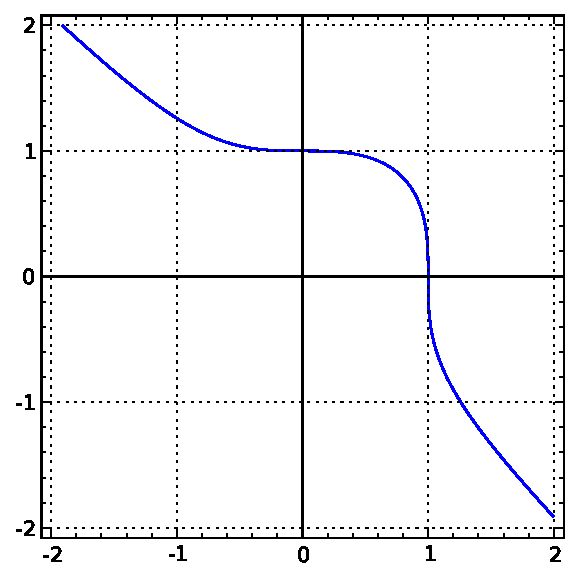
\includegraphics[width=.5\textwidth]{pics/flt3.pdf}
\end{center}
This is an example of an elliptic curve; you should
see some rational points on it---namely $(1,0)$ and $(0,1)$---these
correspond to torsion points on the elliptic curve, and to solutions
to the Fermat equation with $X$ or $Y$ equal to $0$.

For general $n\geq 5$, Fermat's assertion was finally resolved by much modern
work in number theory, culminating with a major theorem of
Andrew Wiles.  The basic strategy, which is useful for
attacking a wide range of Diophantine equations, is as follows.
Given a specific counterexample
$a^n + b^n = c^n$ to Fermat's claim (with say $n$ prime), we associate
an elliptic curve (the ``Frey curve'')
$$
  E: \quad y^2 = x(x-a^n)(x+b^n).
$$
By counting solutions modulo $p$ to the equation that defines this curve (or
any nonsingular curve of the form $y^2=x^3+\alpha x + \beta$ for that matter),
we define an $L$-series
$$
L(E,s) =
\prod_{p \text{ prime}} \frac{1}{1-a_p p^{-s} + \varepsilon(p)\cdot p^{1-2s}}
 = \sum_{n\geq 1} \frac{a_n}{n^s},
$$
where $\varepsilon(p)=1$ if $p\nmid abc$ and $\varepsilon(p)=0$ otherwise,
and $a_p = p+1-\#E(\F_p)$.
Old work of Hasse (and others)
shows that this $L$-series defines a complex analytic
function on some right half plane; people then conjectured (and
subsequently proved!)
that $L(E,s)$ extends to a holomorphic function on all $\C$.
Birch and Swinnerton-Dyer even went so far as to conjecture
that most everything about the arithmetic of $E$
is determined by the leading coefficient of the
Taylor expansion of $L(E,s)$ about $s=1$.

To the $L$-series $L(E,s)$, one can use
Mellin transform to define another complex analytic function
on the upper half plane
$$
f(z) = \sum_{n\geq 1} a_n e^{2\pi i z} = \sum_{n\geq 1} a_n q^n,
$$
where the coefficients $a_n$ here are exactly the same as
in the Dirichlet series representation of $L(E,s)$ above.
Andrew Wiles (and Richard Taylor) proved \cite{wiles:fermat}---using
an ingenious
argument involving an arithmetic analogue of Barry Mazur's
deformation theory---that
$f(z)$ has the property that for
all $2\times 2$ integer matrices
$\gamma$ with determinant $1$ and lower left entry divisible
by $N=\prod_{\ell\mid abc} \ell$, we have
$$
  f(z) dz = f(\gamma(z)) d(\gamma(z)),
$$
where $\gamma$ acts on the upper half plane
via linear fractional transformations.  This function
$f(z)$ is called a weight 2 cuspidal {\em modular form}.

Moreover, using arithmetic with {\em quaternion algebras} and
geometry of modular curves, Ken Ribet had earlier proved that
the coefficients $a_n$ of the expansion of
$f(z)$ must be congruent to the coefficients
of a cuspform of ``level 2'', which is
impossible, since there are no such nonzero forms.
This contradiction proves Fermat's last theorem.

We can explicitly compute with many of the
objects---elliptic curves, modular forms, etc.---appearing
in the discussion above.
For example, we do some computations with the elliptic
curve corresponding to Fermat's equation for exponent $n=3$
(this is {\em not} the corresponding Frey curve, but another
model for $X^3+Y^3=1$)
\begin{lstlisting}
sage: E = EllipticCurve([0,0,1,0,-7]); E
Elliptic Curve defined by y^2 + y = x^3 - 7 over Rational Field
sage: E.anlist(20)
[0, 1, 0, 0, -2, 0, 0, -1, 0, 0, 0, 0, 0, 5, 0, 0, 4, 0, 0, -7, 0]
sage: L = E.lseries(); L
Complex L-series of the Elliptic Curve defined by y^2 + y = x^3
over Rational Field
sage: L(1)
0.588879583428483
sage: L.taylor_series(1, 5)
0.59 + 0.45*z - 0.19*z^2 + 0.0042*z^3 + 0.033*z^4 - 0.018*z^5 + O(z^6)
sage: E.rank() # proves FLT for exponent 3
0
\end{lstlisting}
By computing the ranks of twists of $E$ we can tell whether or
not $E$ has infinitely many rational points over the quadratic
field $\Q(\sqrt{d})$, for various $d$.  Running this code:
\begin{lstlisting}
for d in [-5..5]:
    if d.is_squarefree() and d != 1:
       print d, E.quadratic_twist(d).rank()
\end{lstlisting}
yields:
\begin{lstlisting}
-5 1
-3 0
-2 1
-1 0
2 1
3 0
5 1
\end{lstlisting}
This means, e.g., that in the field $\Q(\sqrt{5})$, generated by
the golden ratio, there are infinitely many triples of coprime integers
$X,Y,Z$ such that $X^3 + Y^3 = Z^3$!

\hw{Travis Scholl}{Explicitly find some of these triples $X,Y,Z$ as above,
by finding an explicit isomorphism between the algebraic
curves $X^3+Y^3=1$ and $y^2+y=x^3-7$, and transferring some points
of infinite order on $y^2+y=x^3-7$ back via this isomorphism.}

And we can explore the $L$-series itself:

\begin{lstlisting}
sage: h = L.dokchitser(prec=200)
sage: complex_plot(h, (-2,3), (-5,5), plot_points=10)  # quite painful
\end{lstlisting}

\begin{center}
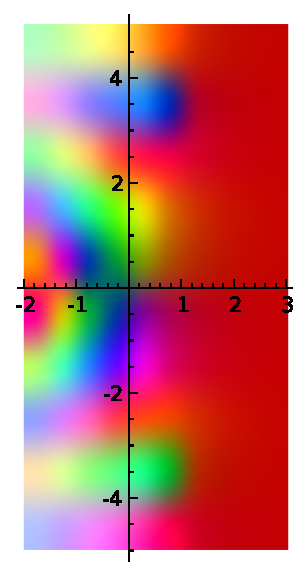
\includegraphics[width=.4\textwidth]{pics/27a-lser1.pdf}
\end{center}

As for the Riemann zeta function, there is a generalized Riemann
Hypothesis, which postulates that the nontrivials zeros of
$L(E,s)$ lie on a line, the line $\Re(s)=1$.
The first few imaginary parts of the nontrivial zeros of $L(E,s)$ are
\begin{lstlisting}
sage: L.zeros(5)
[4.04304401, 6.04893540, 8.21765037, 9.42919921, 10.9087283]
\end{lstlisting}

The general structure of Wiles's approach also generalizes to many other
Diophantine equations.  Instead of obtaining a single congruence with
forms in a space of dimension 0, we instead considers a potential
large collection of spaces of modular forms, which we systematically
compute (e.g., using modular symbols).

\subsection{Failure of Fermat's Last Theorem} %Added by Travis Scholl

There are many rings where Fermat's Last Theorem fails for many values of
$n$. For example consider the ring $\Z[\zeta]$ where $\zeta$ is a primitive
$m$th root of unity with $3 | m$. Then $\xi := \zeta^\frac{m}{3}$ is
a primitive $3$rd root of unity so it satisfies $1+\xi+\xi^2=0$.
From this it is easy to see
$$
(\xi)^{6k+5} + (\xi^2)^{6k+5} = (-1)^{6k+5}
$$
for any non-negative integer $k$. Hence the triple $(\xi,\xi^2,-1)$ satisfies
the Fermat equation $X^{6k+5}+Y^{6k+5}=Z^{6k+5}$ in the ring $\Z[\zeta]$. \\

In general, it is straightforward to construct counterexamples to FLT
of degree $d$ with degree $d$ number fields: \\
Let $d\ge 3$ be a positive integer, and pick any to positive integers
$Y$ and $Z$ with $Y<Z$. Let $K = \Q(\alpha)$, where $\alpha$ obeys
$\alpha^d = Z^d-Y^d \in \Z$. Then clearly $(\alpha,Y,Z)$ is a Fermat triple lying in $K$. \\


\section{The abc Conjecture}
The abc conjecture
concerns triples of coprime positive integers $a,b,c$  such that
$$
a+b = c.
$$
The {\em radical} of an integer $n$ is the product
of the distinct prime divisors of $n$, and the radical
of an abc triple $a,b,c$ is $r=r(a,b,c)=r(abc)$.
For example,
$$
  1 + 8 = 9
$$
has radical $r=2\cdot 3=6$.

\begin{conjecture}[Masser-Oesterl\'{e}]\label{conj:abc}
For every $\eps>0$ there are only finitely many
triples $a,b,c$ of coprime positive integers such
that $a+b=c$ and $r^{1+\eps}\leq c$,
where $r=r(a,b,c)$.
\end{conjecture}

Given $a,b$ it is trivial to find $c$ with $a+b=c$, and
usually the radical $r=r(a,b,c)$ is going to be bigger
than $c$.   A typical example is $a=4$, $b=15$.
We have $c=4+15=19$, and the radical is
$$2\cdot 3\cdot5\cdot19=570 \gg 19.$$
For the radical to be small compared to $c$
is quite special.

Now suppose for the moment that we have a counterexample
to Fermat's Last Theorem (see Section~\ref{sec:fltintro} above),
say
$$
 A^n + B^n = C^n,
$$
with $A,B,C$ coprime positive integers and $n\ge 5$ (say).
Letting $a=A^n, b=B^n, c=C^n$, we have
$$
r(a,b,c) = r(A^n,B^n,C^n) = r(A,B,C) = ABC <C^3 < C^n=c.
$$
According to Conjecture~\ref{conj:abc} (with
any choice of $\eps$), there can be only finitely many such
triples $(A^n, B^n, C^n)$.  In particular, Conjecture~\ref{conj:abc} implies
Fermat's Last Theorem for all sufficiently large $n$.
\footnote{An accepted proof of FLT is known (due to Wiles). There
is no accepted proof of ABC, but there is a claimed one,
which may or may not be right...
\begin{quote}
``The problem with wrong proofs to correct statements is that it is hard to give a counterexample.'' -- Hendrik Lenstra, \url{http://www.ucs.louisiana.edu/~avm1260/lenstra.html}
\end{quote}}

There's much computational work that goes into understanding
and refining the ABC conjecture.  For example,
Lenstra defined a notion of the {\em quality} of
a triple $a+b=c$ to be
$$q(a,b,c) = \frac{\log(c)}{\log(r)}.$$

Here is a Sage interact to compute the quality:
\begin{lstlisting}
@interact
def f(a=3, b=4):
    c = a + b
    print "%s + %s = %s"%(a,b,c)
    v = prod(set(prime_divisors(a) + prime_divisors(b) + prime_divisors(c)))
    q = log(c)/log(v)
    print "quality = ", float(q)
\end{lstlisting}

Notice that if we chose $\eps$ to get equality
in Conjecture~\ref{conj:abc}, then
$q(a,b,c) = 1+\eps$.
As mentioned above, triples $a,b,c$ usually have
very low quality, since
$r$ is typically much bigger than $c$.
However, there are some known triples $a,b,c$ of
high quality, but the ABC conjecture asserts there aren't too
many.  In fact, here is an equivalent version of the ABC conjecture:
\begin{conjecture}
For every $h>1$ there are only finitely many triples
$a,b,c$ with quality bigger than $h$.
\end{conjecture}

The highest quality triple ever found\footnote{See \url{http://www.math.leidenuniv.nl/~desmit/abc/}.} is
$
   2 + 3^{10}\cdot 109 = 23^5,
$
where
$$
q(a,b,c) = \frac{\log(23^5)}{\log(2\cdot 3 \cdot 109 \cdot 23)}
    = 1.62991168412\ldots
$$

Even if you don't believe the ABC conjecture, you might believe this:
\begin{conjecture}[Weak ABC]
Among all $a,b,c$ triples, there is an absolute upper
bound on the quality.
\end{conjecture}

\begin{exercise}
Does the above weaker conjecture imply Fermat's Last Theorem for all sufficiently large exponents $n$?
\end{exercise}

\begin{exercise}
If possible, formulate ABC over number fields in terms of a notion of ``quality''.  See \url{http://www.math.columbia.edu/~goldfeld/ABC-Conjecture.pdf} for a precise statement of ABC over number fields.
What does this imply about FLT over number fields?
\end{exercise}

%added by Hao Chen 10/6/13
In the paper mentioned in Exercise 1.5.5, Goldfeld
formed a slightly different version of ABC:

(ABC')Let $A,B,C$ be nonzero, coprime integers such that
$A+B+C = 0$. Let $N = \prod_{p \mid ABC} p$.
Then for every $\epsilon >0$, there exists $\kappa(\epsilon)>0$
such that
\[ \max(|A|,|B|,|C|) < \kappa(\epsilon) N^{1+\epsilon} \]
The first question is if this conjecture is equivalent
to ABC. One sees that ABC implies ABC': indeed, fix
any $\epsilon >0$, then $\kappa$ can be chosen to be any number greater than $\max\{ \frac{\max\{|A|,|B|,|C|\}}{N^{1+\epsilon}}\}$. This maximum taken over a set is finite since by ABC all but finitely many element in
this set is smaller than 1. \\

Proof that ABC' implies ABC: Fix $\epsilon > 1$,
choose $\delta$ s.t. $\epsilon > \delta > 1$, then
by ABC', there exists some positive constant $\kappa(\delta)$
such that $\max(|A|,|B|,|C|) < \kappa(\delta) N^{1+\delta}$
holds for all triples. Now for any triple s.t. $N^{1+\epsilon} < \max(|A|,|B|,|C|)$ we have
$N^{1+\epsilon}< N^{1+\delta}$, which can only hold for
finitely many $N$. Hence $N$ is bounded above, and we see
from ABC' that $\max(|A|,|B|,|C|)$ is bounded above. So
there's finitely many such triples.



\subsection{Infinitely many triples with quality greater than $1$}
For $p$ an odd prime and $n\geq 1$ an integer, consider the $a,b,c$ triple
$$
a = 1,\qquad b = 2^{p(p-1)n}-1, \qquad c = 2^{p(p-1)n}.
$$
Since $\varphi(p^2)=p(p-1)$ is the order of $(\Z/p^2\Z)^*$,
we have $2^{p(p-1)n}\equiv 1 \pmod{p^2}$,
so $p^2 \mid b$.
Thus
$$
 r = r(a,b,c) = 1 \cdot p \cdot\text{(other stuff from $b$)} \cdot 2
     \leq \frac{2b}{p} < b < c,
$$
so
$$
 q(a,b,c) = \frac{\log(c)}{\log(r)} > 1.
$$
Here is a Sage interact to compute $a,b,c$ as above, along with their quality.
Note that if you put at all largve values in for either $n$ or $p$,
then the resulting numbers are huge, and the computation of the quality
(as implemented) will take forever.
\begin{lstlisting}
@interact
def f(p=3, n=1):
    if not is_prime(p) or p<=2:
        print "p must be an odd prime!"
    if n < 1:
        print "n must be >= 1"
    a = 1
    b = 2^(p*(p-1)*n) - 1
    c = 2^(p*(p-1)*n)
    print "%s + %s = %s"%(a,b,c)
    print "(now computing quality...)"
    sys.stdout.flush()
    v = prod(set(prime_divisors(a) + prime_divisors(b) + prime_divisors(c)))
    q = log(c)/log(v)
    print "quality = ", float(q)
\end{lstlisting}

\subsection{Triples with Quality at least $1.4$}
The following is a plot of the number of abc triples with $c\leq 10^x$
and quality at least $1.4$, drawn on a log scale,
where $x\leq 10^{18}$.  This data was computed by the ABC@HOME project.
\begin{center}
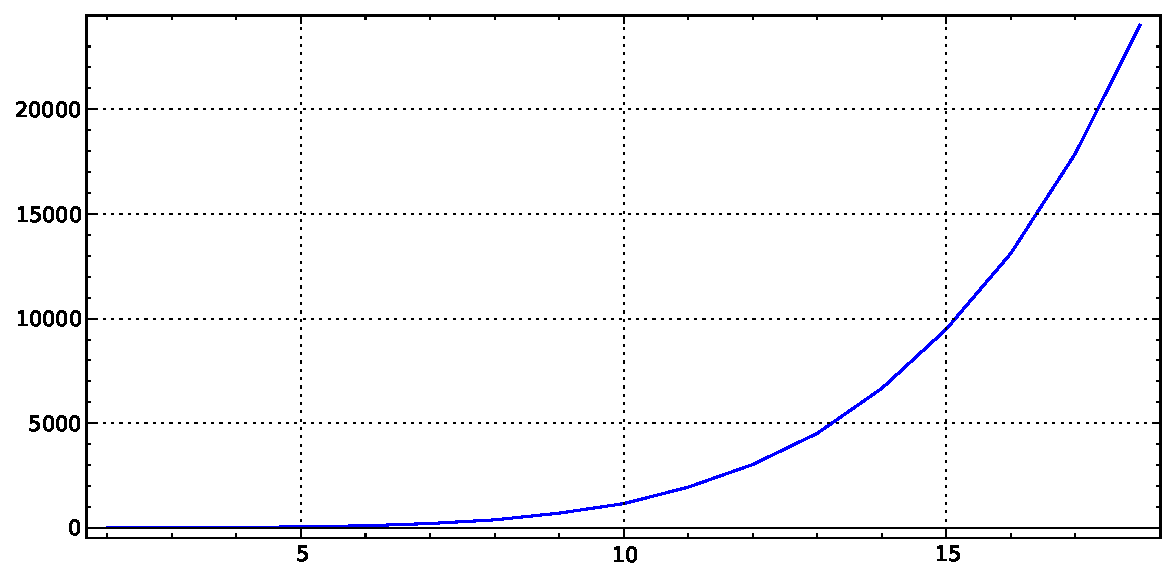
\includegraphics[width=.7\textwidth]{pics/abcplot.pdf}
\end{center}

The (strong) ABC conjecture asserts that the blue line is bounded above!
As is typical is typical with most questions in "asymptotic number theory",
the numerical data suggests---to the naive observer---the exact opposite.
See \cite{bmsw:bulletins} for an article about this sort of tension in
another context:
\begin{quote}
``We have a network of heuristics and conjectures regarding rational points, and we have massive data accumulated to exhibit instances of the phenomena. Generally, we would expect that our data supports our conjectures; and if not, we lose faith in our conjectures. But here there is a somewhat more surprising interrelation between data and conjecture: they are not exactly in open conflict one with the other. We discuss various aspects of this story, including recent heuristics and data that attempt to resolve this mystery.''
\end{quote}

{\bf Student Project Idea: } {\em Completely forget about the ABC
conjecture, pretend you are an applied mathematician,
and model the function that counts the number of ABC
triples of quality $q$ up to $10^x$.}
\begin{enumerate}
\item Beg, barrow, or steel the complete dataset from the ABC@Home
project.  This could be pretty challenging, since currently their
site is down with ``{\tt Warning: mysql\_pconnect(): Too many connections in /data/project/abc/html/inc/db.inc on line 39...}''.  That said, I know the people who run this site,
and we can contact them directly.
\item For a few hundred values of $q$ with $1\leq q\leq 1.67$,
use the data to "compute or plot" the function
$$
f_q(x) = \#\{\text{number of ABC-triples with $c<10^x$
of quality $\geq q$}\}.
$$
The plot will look like the blue curve above.
\item
Use various models of your choosing to find a smooth
function that best fits that curve?  Your smooth
function will be parametrized by $q$, i.e., you get
a different function for each value of $q$.
I don't have any idea what sort of function to expect.
A polynomial?  Exponential?  Something else?  Note that
according to the ABC conjecture, the function $f_q(x)$
is supposed to be {\em bounded above} for each $q>1$!
(However, just pretend you don't know about that and you're
a physicist or something....)
\item What happens if you let the parameter $q$
in the above model go to $\infty$?
\item Can you find a different model for $f_q(x)$ that
{\em is} bounded above (hence consistent with the ABC
conjecture), and also fits the data?
\end{enumerate}

The above seems to me to be the most obvious first thing to
do if one had computing power and wanted to make the ABC
conjecture in the first place.  However, the data to do the
above computation wasn't available until very recently,
so maybe nobody did it (which I find sort of shocking if true).

% Bharath added this section
\section{Some consequences of the ABC conjecture}

\begin{enumerate}
\item In \cite{ichimura1998note}, assuming the generalized ABC conjecture for number fields, H. Ichimura shows that for a given real quadratic field $k$, there exists infinitely many prime numbers $p$ such that the Iwasawa $\lambda$-invariant.
This is closely related to Greenberg's conjecture.
\item In \cite{elkies1991abc}, N. Elkies shows that the generalized ABC conjecture for number fields implies the Mordell conjecture.
\item
\end{enumerate}


\section{Public-key Cryptography}


\begin{quote}
``Nowadays, when a Number Theorist applies for a grant, he says
that Number Theory is used in cryptography, and so doing Number
Theory is good for National Security. Back then, since it was
before the discovery of America, they said Number Theory is
used in music. But I won't comment on the progress of
civilization since then.''\\-- Hendrik Lenstra,\\ \url{http://www.ucs.louisiana.edu/~avm1260/lenstra.html}
\end{quote}


Public-key cryptography involves many of the same ideas and tools
as the rest of computational number theory, and so in this book
we will consider it on an equal footing.
In particular, we will consider the RSA cryptosystem, whose
security relies on the difficulty of factoring integers,
and also elliptic curve-based cryptosystems
such as ElGamal and elliptic curve Diffie-Hellman.

There are two intimately related sides to cryptography:
creating methods to send encrypted messages,
and cracking proposed encryption methods.
It's extremely difficult to be good at
creating methods for encrypting messages, but
bad at attacking them, since one must be very aware of
attack techniques in order to guard against them.
It's probably less important to be good at making encryption
systems if you want to be good at cracking them.
It is natural that the typical cryptography group at a big
company would put more effort into
creating and implementing cryptosystems than into attacking them,
since they
have little commercial motivation for investing billions
into attacking cryptosystems,
and publicity about them doing so probably wouldn't look
good (and indeed, such attack technology might have legal implications).
\begin{quote}
``Former NSA technology boss Prescott Winter has a word for the kind of security he sees even at large, technologically sophisticated companies: Appalling''\\
 -- \url{http://tinyurl.com/pgb45j8}, Slashdot, Oct 3, 2013.
\end{quote}

For the cryptography aspect of this course, we'll consider the cryptosystems above, and some of the attacks on them, and how all of this work
has a deep interplay with many other objects we consider.

% NEWS: https://news.ycombinator.com/item?id=6506120

\subsection{The Standard Protocols}
To get started, let's quickly go over a couple of bog
standard public-key cryptography protocols: Diffie-Hellman,
RSA, and elliptic curve ElGamal.

\subsubsection{Diffie-Hellman}
The Diffie-Hellman key exchange protocol enables two
programs $A$ and $B$ to agree on a common secret in full view of an
adversary.   For example, Diffie-Hellman (but on an elliptic curve)
is used  when you connect your web browser to the
\url{https://cloud.sagemath.com} website in order to agree
on a secret key that is used to encrypt all further data.

Here's how it works.
\begin{enumerate}
\item Programs $A$ and $B$ agree on a prime number $p$ and a primitive
root $g$ modulo $p$, i.e., a number that generates $(\Z/p\Z)^*$.
\item Program $A$ compute a random number $a$ and program
$B$ computes a random number $b$.
\item Program $A$ sends $g^a\pmod{p}$ and program $B$
sends $g^b\pmod{p}$.
\item Program $A$ and program $B$ compute the secret
$$
   s = (g^a)^b\pmod{p} = (g^b)^a\pmod{p}.
$$
\end{enumerate}
One subtlety is that there is a fast algorithm to
compute $g^n\pmod{p}$ -- to do this, write $n$
in binary, and compute $g\cdots g$ ($n$ times)
by a couple of repeated squarings, reducing
modulo $p$ at each step... which is {\em easy}.

The main theoretical assumption one makes is that given $g^n\pmod{p}$
and $g\pmod{p}$ it is ``difficult'' to compute $n$, i.e., to find
$\log_g(g^n \pmod{p})$.  This is the {\em discrete log problem}.
There are some primes $p$ for which this assumption is obviously
false.  For example, if $p-1$ factors as a product of many small
numbers, then solving the discrete log problem in $(\Z/p\Z)^*$ is
no more difficult than solving it in groups with these much smaller
orders, hence easy.   So, if when using Diffie-Hellman, it is critical
to check that $p-1$ doesn't factor too much; the best you can hope
for is that $p-1 = 2q$, with $q$ prime, and this is what people
often use.

Once you commit to seriously using Diffie-Hellman modulo a prime, you have
to worry about how big to make $p$.  If you make $p$ enormous, then
everything takes more memory and is slower.  For example, for large $p$
establishing a connection to \url{https://cloud.sagemath.com} might
take so much time (seconds!) that you'll just loose patience.  To decide
how big a $p$ to take, you basically have to learn about algorithms for
attacking the discrete log problem, look at what challenge problems
people have solved in practice, then bet the farm on a particular
choice size of $p$.    In practice, people usually trust organizations
such as NIST (which is advised by NSA, which knows a thing or two)
to make the decisions for them.

\begin{exercise}
How big of primes $p$ to people actually use?
\end{exercise}

There is an algorithm called "baby-step giant-step" which can solve
the discrete logarithm mod $p$ using time and space $O(\sqrt{p})$; we'll
consider this algorithm in more detail later, since it is extremely
important in computational  number theory.


The Diffie-Hellman key exchange is amenable to the {\em man-in-the-middle
attack}, where an adversary intercepts all transmissions, and
agrees on two different secrets, one with program $A$ and a {\em different
secret} with program $B$.  Then the adversary decrypts/encrypts
all traffic between $A$ and $B$.  This is not theoretical -- exactly
this attack is used successfully
in practice on the Internet (see recent news articles).


\subsubsection{RSA}
The RSA cryptosystem allows a program $A$ to publish a public key
for all to see. Any program $B$ can then send $A$ a message that is encrypted
using this public key.  Also, $A$ can sign documents
using their corresponding private key, and $B$ can use
$A$'s public key to verify that indeed $A$ signed the document.
This RSA solves two problems: (1) being able to encrypt a message to $A$
without any specific activity on $A$'s part (unlike with Diffie-Hellman),
and (2) being able to digitally sign a document.
The main issue is that $B$ has to trust that $A$'s public key is...
really $A$'s public key, and in practice this is a major pain.

Here's how it works.
\begin{enumerate}
\item Program $A$ chooses two prime numbers $p\neq q$
and computes $n=pq$, computes $\varphi(n) = (p-1)(q-1)$,
and chooses an integer $e>1$ that is coprime to $\varphi(n)$.
Program $A$ then publishes $(n, e)$.  Also, program $A$
computes $d$ such that $ed\equiv 1\pmod{\varphi(n)}$.
\item Program $B$ encrypts a message $m\pmod{n}$ to $A$
by computing $m^e\pmod{n}$.  (We assume the message $m$
is coprime to $n$.)
\item Program $A$ decryptes the message $m^e\pmod{n}$
by computing $m=(m^e)^d\pmod{n}$, where we use that
$\varphi(n)$ is the order of $(\Z/n\Z)^*$.
\item Also, if program $A$ wishes to sign a message $m$,
then program $A$ publishes $m$ and $m^d\pmod{n}$.
\item Program $B$ can verify that program $A$ signed $m$
by computing $(m^d)^e\pmod{n}$ and checking that this
equals $m$.
\end{enumerate}

The security of RSA relies on the secret $d$, which is easy
to compute if you know $\vphi(n)$.  However, knowing $\vphi(n)$
requires factoring $n$, which seems---as far as we know---to
be difficult in general.   All the same remarks as for Diffie-Hellman
apply above; in order to know how big to choose $n$, you need
to be intimately familiar with approaches to factoring large integers
$n$, or you look at what people have done and trust expert recommendations.
As always, there is a tradeoff between speed and security.

\begin{exercise}
Install the gpg program (``gnu privacy guard''), generate an RSA
key, and post the public part of it on your webpage, so that other
people can send you secret messages.  What bitsize did you choose?
\end{exercise}


\subsubsection{ElGamal}

\subsection{The Bitcoin Elliptic Curve}

http://www.extremetech.com/computing/168139-fbi-unable-to-seize-600000-bitcoins-from-silk-road-operator

http://www.coindesk.com/capital-one-closes-bank-account-bitcoin/

\subsection{How to find a primitive root mod $p$}

First, let us consider an easy example. Let us assume that the prime $p$ satisfies the relation $p-1=2\cdot q$, where $q$ is also a prime number. Now, the order of any element in $(\Z/p\Z)^\times$ is either $1$, $2$, $q$ or $2 \cdot q$. Now, $-1$ is not a square in $(\Z/p\Z)^\times$, since $4$ does not divide $p-1$. Hence, either $2$ or $-2$ (and exactly one of them) will be a generator for the cyclic group $(\Z/p\Z)^\times$. So, it suffices to computee $2^q$ and check if it equals $1$ or $-1$.



\chapter{Prime Numbers}

Main unsolved problem: the Riemann Hypothesis



\section{Infinitely many primes}
\section{The Prime number theorem}
\section{The Riemann hypothesis}
\section{The Explicit Formula}
\section{Generalizations to number fields}


\chapter{Arithmetic of Number Fields}
Main unsolved problem: class number 1 fields

\section{Class groups}
\section{The Gauss class number problem}
\section{Number fields of class number 1}
 (Cohen-lenstra, Bharghava)



\chapter{Diophantine Equations: Fermat and ABC}
Main unsolved problem: ABC conjecture

\section{Fermat's Last Theorem}
\section{The ABC Conjecture}
\section{Generalized Fermat equations}



\chapter{Elliptic Curves}
Important unsolved problem: the BSD conjecture (computing Mordell-Weil groups)

\section{The Group law}
\section{The Mordell-Weil theorem}
\section{Mazur's classification of torsion subroups}
\section{The $L$-series}
analytic continuation and functional equation (modularity)
\section{The Birch and Swinnerton-Dyer conjecture}
\section{The Hasse bound}
\section{The Explicit Formula}



\chapter{Modular Forms}
Important unsolved problem: modularity of elliptic curves
over totally real fields

\section{Ramanujan bound}
\section{Galois representations attached to modular forms}
\section{Modularity of elliptic curves}




\chapter{Public-key Cryptography}

Important unsolved problem: how difficult is the discrete log problem?

\section{Protocols: Diffie-Hellman, RSA, ElGamal, ...}
\section{Discrete log problem (baby-step, giant-step)}


\bibliographystyle{amsalpha}
\bibliography{biblio}

\end{document}

%sagemathcloud={"zoom_width":140}
